\documentclass[letterpaper,12pt,preprint]{hack_aastex}

% Colors.
\usepackage{amsmath}
\usepackage{color}
\usepackage[pagebackref=false]{hyperref}
\definecolor{linkcolor}{rgb}{0,0,0.25}
\hypersetup{colorlinks=true,linkcolor=linkcolor,citecolor=linkcolor,
            filecolor=linkcolor,urlcolor=linkcolor}

\usepackage[para]{footmisc}
\urlstyle{sm}

\usepackage{epsfig}
\usepackage{graphicx}
\setlength{\headheight}{2ex}
\setlength{\headsep}{2ex}

\usepackage{multicol}

\newcommand{\dd}{\,\mathrm{d}}
\newcommand{\bvec}[1]{{\ensuremath{{\boldsymbol{#1}}}}}
\newcommand{\transpose}[1]{{#1}^{\!\mathsf{T}}}
\newcommand{\inverse}[1]{{#1}^{-1}}


%----- exact 1-in margins
% NB: headheight and headsep MUST exist and be set
\setlength{\textwidth}{6.5in}
\setlength{\textheight}{9in}
\addtolength{\textheight}{-1.0\headheight}
\addtolength{\textheight}{-1.0\headsep}
\setlength{\topmargin}{-2em}
\addtolength{\textheight}{-1.0\topmargin}
\setlength{\oddsidemargin}{0.0in}
\setlength{\evensidemargin}{0.0in}

%----- typeset certain kinds of words
\newcommand{\observatory}[1]{\textsl{#1}}
\newcommand{\package}[1]{\textsf{#1}}
\newcommand{\project}[1]{\package{#1}}
\newcommand{\an}{\package{Astrometry.net}}
\newcommand{\NASA}{\observatory{NASA}}
\newcommand{\JWST}{\observatory{JWST}}
\newcommand{\Kepler}{\observatory{Kepler}}
\newcommand{\kepler}{\Kepler}
\newcommand{\Ktwo}{\observatory{K2}}
\newcommand{\ktwo}{\Ktwo}
\newcommand{\KT}{\Ktwo}
\newcommand{\PLATO}{\observatory{PLATO}}
\newcommand{\MAST}{\observatory{MAST}}
\newcommand{\EA}{\observatory{Exoplanet Archive}}
\newcommand{\TESS}{\observatory{TESS}}
\newcommand{\galex}{\observatory{GALEX}}
\newcommand{\Spitzer}{\observatory{Spitzer}}
\newcommand{\gaia}{\observatory{Gaia}}
\newcommand{\Gaia}{\gaia}
\newcommand{\lsst}{\observatory{LSST}}
\newcommand{\sdss}{\observatory{SDSS}}
\newcommand{\latin}[1]{\textit{#1}}
\newcommand{\eg}{\latin{e.g.}}
\newcommand{\etal}{\latin{et~al.}}
\newcommand{\etc}{\latin{etc.}}
\newcommand{\ie}{\latin{i.e.}}
\newcommand{\vs}{\latin{vs.}}

\newcommand{\doi}[2]{\href{http://dx.doi.org/#1}{\emph{#2}}}
\newcommand{\ads}[2]{\href{http://adsabs.harvard.edu/abs/#1}{\emph{#2}}}
\newcommand{\arxiv}[1]{\href{http://arxiv.org/abs/#1}{arXiv:#1}}

%----- stuff for this proposal in particular.
\newcommand{\kplr}{\package{kplr}}
\newcommand{\PLM}{\package{PLM}}
\newcommand{\OWL}{\package{OWL}}
\newcommand{\George}{\package{George}}
\newcommand{\kpsf}{\package{kpsf}}
\newcommand{\emcee}{\package{emcee}}
\newcommand{\GitHub}{\package{GitHub}}
\newcommand{\KIC}{\textsl{KIC}}
\newcommand{\KOI}{\textsl{KOI}}

%----- typeset journals
% \newcommand{\aj}{Astron.\,J.}
% \newcommand{\apj}{Astrophys.\,J.}
% \newcommand{\apjl}{Astrophys.\,J.\,Lett.}
% \newcommand{\apjs}{Astrophys.\,J.\,Supp.\,Ser.}
% \newcommand{\mnras}{Mon.\,Not.\,Roy.\,Ast.\,Soc.}
% \newcommand{\aap}{Astron.\,\&~Astrophys.}

%----- Tighten up paragraphs and lists
\setlength{\parskip}{0.0ex}
\setlength{\parindent}{0.2in}
\renewenvironment{itemize}{\begin{list}{$\bullet$}{%
  \setlength{\topsep}{0.0ex}%
  \setlength{\parsep}{0.0ex}%
  \setlength{\partopsep}{0.0ex}%
  \setlength{\itemsep}{0.0ex}%
  \setlength{\leftmargin}{1.5\parindent}}}{\end{list}}
\newcounter{actr}
\renewenvironment{enumerate}{\begin{list}{\arabic{actr}.}{%
  \usecounter{actr}%
  \setlength{\topsep}{0.0ex}%
  \setlength{\parsep}{0.0ex}%
  \setlength{\partopsep}{0.0ex}%
  \setlength{\itemsep}{0.0ex}%
  \setlength{\leftmargin}{1.5\parindent}}}{\end{list}}

%----- mess with paragraph spacing!
\makeatletter
\renewcommand\paragraph{\@startsection{paragraph}{4}{\z@}%
                                    {1ex}%
                                    {-1em}%
                                    {\normalfont\normalsize\bfseries}}
\makeatother

%----- Special Hogg list for references
  \newcommand{\hogglist}{%
    \rightmargin=0in
    \leftmargin=0.25in
    \topsep=0ex
    \partopsep=0pt
    \itemsep=0ex
    \parsep=0pt
    \itemindent=-1.0\leftmargin
    \listparindent=\leftmargin
    \settowidth{\labelsep}{~}
    \usecounter{enumi}
  }

%----- side-to-side figure macro
%------- make numbers add up to 94%
 \newlength{\figurewidth}
 \newlength{\captionwidth}
 \newcommand{\ssfigure}[3]{%
   \setlength{\figurewidth}{#2\textwidth}
   \setlength{\captionwidth}{\textwidth}
   \addtolength{\captionwidth}{-\figurewidth}
   \addtolength{\captionwidth}{-0.02\figurewidth}
   \begin{figure}[htb]%
   \begin{tabular}{cc}%
     \begin{minipage}[c]{\figurewidth}%
       \resizebox{\figurewidth}{!}{\includegraphics{#1}}%
     \end{minipage} &%
     \begin{minipage}[c]{\captionwidth}%
       \textsf{\caption[]{\footnotesize {#3}}}%
     \end{minipage}%
   \end{tabular}%
   \end{figure}}

 \newcommand{\ssfiguretwo}[4]{%
   \setlength{\figurewidth}{#3\textwidth}
   \setlength{\captionwidth}{\textwidth}
   \addtolength{\captionwidth}{-\figurewidth}
   \addtolength{\captionwidth}{-0.02\figurewidth}
   \begin{figure}[htb]%
   \begin{tabular}{cc}%
     \begin{minipage}[c]{\figurewidth}%
       \resizebox{\figurewidth}{!}{\includegraphics{#1}}\\
       \resizebox{\figurewidth}{!}{\includegraphics{#2}}%
     \end{minipage} &%
     \begin{minipage}[c]{\captionwidth}%
       \textsf{\caption[]{\footnotesize {#4}}}%
     \end{minipage}%
   \end{tabular}%
   \end{figure}}

%----- top-bottom figure macro
 \newlength{\figureheight}
 \setlength{\figureheight}{0.75\textheight}
 \newcommand{\tbfigure}[2]{%
   \begin{figure}[htp]%
   \resizebox{\textwidth}{!}{\includegraphics{#1}}%
   \textsf{\caption[]{\footnotesize {#2}}}%
   \end{figure}}

%----- deal with pdf page-size stupidity
\special{papersize=8.5in,11in}
\setlength{\pdfpageheight}{\paperheight}
\setlength{\pdfpagewidth}{\paperwidth}

% no more bad lines!
\sloppy\sloppypar

% A better underline!
% tex.stackexchange.com/questions/36894/underline-omitting-the-descenders
\usepackage[T1]{fontenc}
\usepackage[latin1]{inputenc}
\usepackage{soul}
% \usepackage{xcolor}
\usepackage{xparse}
\makeatletter
\ExplSyntaxOn
\cs_new:Npn \white_text:n #1
  {
    \fp_set:Nn \l_tmpa_fp {.01}
    \fp_mul:Nn \l_tmpa_fp {#1}
    \llap{\textcolor{white}{\the\SOUL@syllable}\hspace{\fp_to_decimal:N \l_tmpa_fp em}}
    \llap{\textcolor{white}{\the\SOUL@syllable}\hspace{-\fp_to_decimal:N \l_tmpa_fp em}}
  }
\NewDocumentCommand{\whiten}{ m }
    {
      \int_step_function:nnnN {1}{1}{#1} \white_text:n
    }
\ExplSyntaxOff

\NewDocumentCommand{ \varul }{ D<>{5} O{0.2ex} O{0.1ex} +m } {%
\begingroup
\setul{#2}{#3}%
\def\SOUL@uleverysyllable{%
   \setbox0=\hbox{\the\SOUL@syllable}%
   \ifdim\dp0>\z@
      \SOUL@ulunderline{\phantom{\the\SOUL@syllable}}%
      \whiten{#1}%
      \llap{%
        \the\SOUL@syllable
        \SOUL@setkern\SOUL@charkern
      }%
   \else
       \SOUL@ulunderline{%
         \the\SOUL@syllable
         \SOUL@setkern\SOUL@charkern
       }%
   \fi}%
    \ul{#4}%
\endgroup
}
\makeatother


% Underline paragraph titles
\usepackage[explicit]{titlesec}
\titleformat{\paragraph}[runin]
    {\normalfont\normalsize\bfseries}{\theparagraph}{1em}
    {\varul{#1}}

\pagestyle{myheadings}
\markright{\textsf{\footnotesize %
                   The search for extragalactic exoplanets / %
                   Hogg, Price-Whelan \& Foreman-Mackey}}

% Single-spacing.
\def\baselinestretch{1.0}

\begin{document}

The current.

{\bf We propose to target the brightest likely members of the Sagittarius
stellar stream that fall in the field-of-view of Campaign 8 and search for hot
Jupiters transiting these stars.}

\paragraph{Target selection}

The Sagittarius (Sgr) stream is the most massive and prominent stellar tidal stream observed in the halo of the Milky Way. Stars associated with the stream (via kinematics and chemical abundances) fully encircle the Galaxy and span heliocentric distances of $\approx$15 kpc to $\approx$100 kpc. The footprint of \KT\ fields 8 and 10 overlap with regions of the stream previously detected in K/M giant and F turnoff stars \citep{Majewski:2003, Yanny:2009} at distances of $\approx$20--30 kpc. Though this is an order of magnitude farther than any of the known transiting exoplanets, the stream is one of the closest hosts of extragalactic stars --- thus, the Sgr stream represents a unique opportunity to detect the first exoplanet formed outside of our own Galaxy.

We select M giant candidates using the Two Micron All Sky Survey \citep[2MASS; ][]{Skrutskie:2006} photometry provided in the \KT\ field catalogs\footnote{\url{https://archive.stsci.edu/k2/catalogs.html}} following the selection criteria used in \cite[][hereafter M03]{Majewski:2003}, with slight modifications. We first use the dust reddening measurements of \cite{Schlafly:2011} to de-redden the observed magnitudes (following the conversion of E(B-V) to the 2MASS bandpasses used in M03); for this procedure, we assume all stars are at sufficiently large distances and are therefore behind the dust (an invalid assumption for dwarf stars). We select all point source targets from this catalog by requiring that \texttt{Objtype == `STAR'}: Figures~\ref{fig:field8} and \ref{fig:field10} show all point sources (black markers) in color-magnitude (left) and color-color (right) space for field 8 and 10, respectively. To select the M giant candidates, we first require that either the proper motion in any component is small ($|\mu_\alpha |,|\mu_\delta | < 10~{\rm mas}~{\rm yr}^{-1}$) or that the proper motion is unmeasured. We then use the following (unrestrictive) selection criteria to isolate M giant candidates:
\begin{align} % get outta here with yr eqn arrays
	1.1 &> (J-K_s)_0 > 0.85 \\
	13.1 &> K_s > 10.5\\
	(J-H)_0 &< 0.561\,(J-K_s)_0 + 0.34\\
	(J-H)_0 &> 0.5\,(J-K_s)_0 + 0.2\\
	(J-H)_0 &> -0.4\,(J-K_s)_0 + 1.1
\end{align}
where the first color cut is designed to select M type stars, the $K_s$ magnitude limits are designed to only select would-be M giants in the distance range $\approx$15--40 kpc, and the other color cuts are to limit contamination from dwarf stars \citep[e.g.,][]{Majewski:2003}. For selection in field 10, we instead use the magnitude range $14 > K_s > 12$ because the stream is more distant ($d_\odot \approx 60$ kpc). Over-plotted on Figures~\ref{fig:field8}--\ref{fig:field10} in larger (blue) markers are the targets that pass these criteria, along with the selection window (in color-color space). There are 46 targets in field 8 and 202 targets in field 10. Because the targets in field 10 are fainter, there is more contamination with dwarfs.

\begin{figure*}[p]
\begin{center}
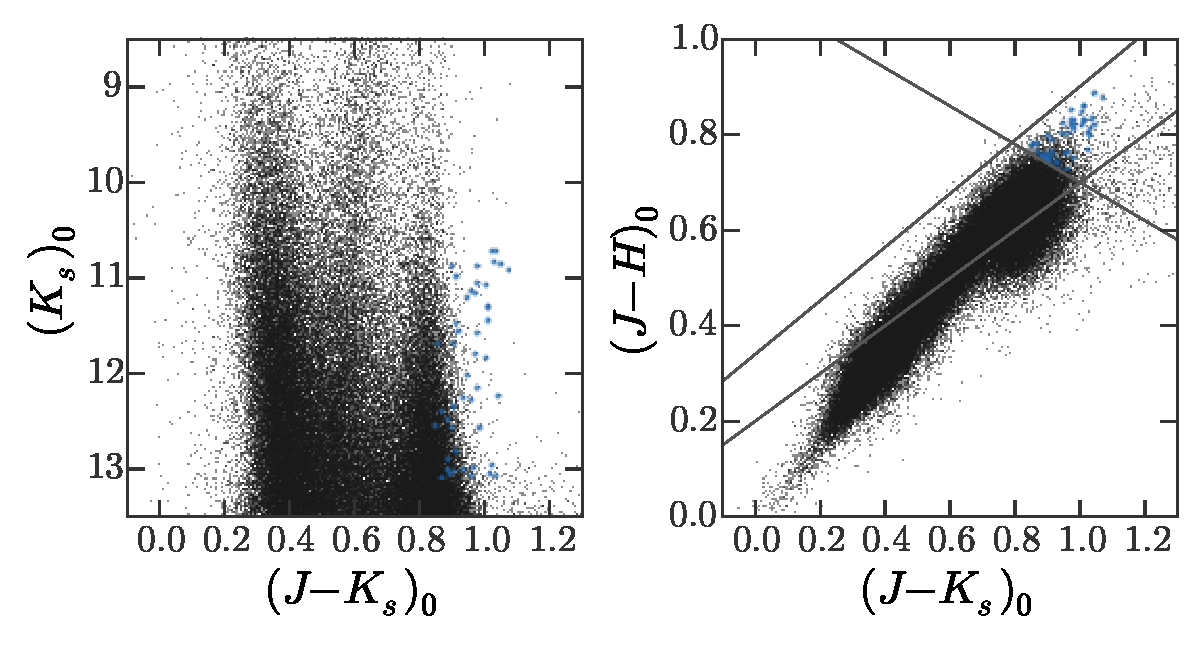
\includegraphics[width=\textwidth]{fig1.pdf}
\caption{} 
\label{fig:field8}
\end{center}
\end{figure*}

\begin{figure*}[p]
\begin{center}
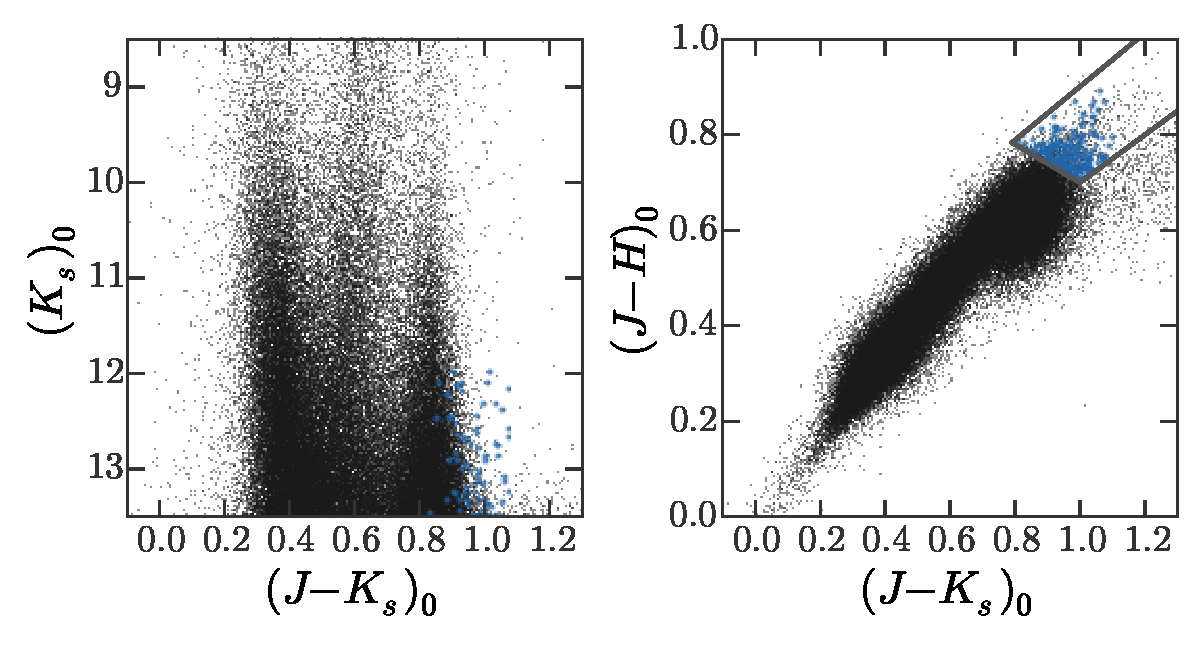
\includegraphics[width=\textwidth]{fig2.pdf}
\caption{} 
\label{fig:field10}
\end{center}
\end{figure*}

TODO: proposed follow-up to get RVs

% Majewski: http://adsabs.harvard.edu/abs/2003ApJ...599.1082M
% Yanny: http://adsabs.harvard.edu/cgi-bin/bib_query?arXiv:0905.4502
% Skrutskie: http://adsabs.harvard.edu/abs/2006AJ....131.1163S
% Schlafly: http://adsabs.harvard.edu/abs/2011ApJ...737..103S

\paragraph{Transit search methodology}

We have developed a method for searching for transit signals using the \KT\
data products and this method resulted in the first systematic catalog of
transiting exoplanets from \KT\ \citep{Foreman-Mackey:2015}.
This method is robust to the systematic variability of the light curves
introduced by instrumental effects but it is susceptible to overfitting when
applied to the light curves of intrinsically variable stars
\citep{Montet:2015}.
Since giant stars have higher amplitude variability, it is necessary to
augment the light curve noise model with a term accounting for the
contribution from the intrinsic variability of the star.
It has been demonstrated that a Gaussian Process
\citep[GP;][]{Rasmussen:2006, Ambikasaran:2014} is a good effective
model for this stochastic variability \citep{Barclay:2015}.
In our original transit search procedure, we phrased the problem as linear
regression \citep{Foreman-Mackey:2015} where the light curve $\bvec{f}$ is
modeled as
\begin{eqnarray}
\bvec{f} &=& \bvec{B}\,\bvec{w} + \bvec{m} + \mathrm{noise}
\end{eqnarray}
where $\bvec{B}$ is a set of eigen light curves (ELCs), $\bvec{m}$ is a
transit model, and the linear weights $\bvec{w}$ are marginalized out in the
computation.
This model can equivalently be written as a GP \citep{Rasmussen:2006}
\begin{eqnarray}
\bvec{f} &\sim& \mathcal{N} (\bvec{m},\,
\bvec{\Sigma} + \bvec{B}\bvec{\Lambda}\bvec{B}^\mathrm{T})
\end{eqnarray}
where $\bvec{\Sigma}$ is the diagonal matrix of measurement variances and
$\bvec{\Lambda}$ is the diagonal matrix of the prior variances on the ELC
weights.
This means that a temporal model for the stochastic stellar variability can
also be included
\begin{eqnarray}
\bvec{f} &\sim& \mathcal{N} (\bvec{m},\,
\bvec{\Sigma} + \bvec{B}\bvec{\Lambda}\bvec{B}^\mathrm{T} + \bvec{K})
\end{eqnarray}
where the elements $K_{ij}$ of $\bvec{K}$ are given by the covariance function
$k(t_i,\,t_j)$.

\paragraph{Estimated planet yield} blah.

\paragraph{The age distribution of the Sagittarius stream}

blah


% \ssfigure{../figures/period.pdf}{0.4}{%
% The posterior probability density for the period
% of a Neptune-sized transiting planet with a $300\,\mathrm{day}$ orbital period
% injected into the \Kepler\ light curve for a relatively bright (\Kepler\
% magnitude $13.5$) G-dwarf.
% \emph{Top:} The light curve---de-trended using a median filter after the
% injection---centered on the transit.
% The data are shown as black points and the lines are $50$ posterior
% predictions for light curve.
% \emph{Bottom:} The Markov Chain Monte Carlo estimate of the posterior
% constraint on the period of the orbit given this single transit.
% The vertical gray line indicates the true injected period.
% To produce this measurement, I assumed that the stellar mass and radius were
% known to $10\%$ and chose a beta function prior on the eccentricity
% \citep{ecc-prior}.
% This distribution is covariant with the stellar parameters, eccentricity, and
% impact parameter and in this figure, I marginalized over these effects.
% \label{fig:period}}

\begin{multicols}{2}
{\centering\bf REFERENCES\par}
\vspace{0.2em}
\begin{thebibliography}{}%
\raggedright\raggedbottom\scriptsize\setlength{\parskip}{-0.5em}%

\bibitem[Ambikasaran \etal(2014)]{Ambikasaran:2014}
Ambikasaran, S., Foreman-Mackey, D., Greengard, L., Hogg, D.~W.,
\& O'Neil, M.\ 2014, \arxiv{1403.6015}

\bibitem[Barclay \etal(2015)]{Barclay:2015}
Barclay, T., Endl, M., Huber, D., Foreman-Mackey, D., \etal\ 2015, \apj, 800,
46

\bibitem[Foreman-Mackey \etal(2014)]{Foreman-Mackey:2014}
Foreman-Mackey, D., Hogg, D.~W., \& Morton, T.~D.\ 2014, \apj, 795, 64

\bibitem[Foreman-Mackey \etal(2015)]{Foreman-Mackey:2015}
Foreman-Mackey, D., Montet, B.~T., Hogg, D.~W., \etal\ 2015, \arxiv{1502.04715}

\bibitem[Montet \etal(2015)]{Montet:2015}
Montet, B.~T., Morton, T.~D., Foreman-Mackey, D., \etal\ 2015,
\arxiv{1503.07866}

\bibitem[Rasmussen \& Williams(2006)]{Rasmussen:2006}
Rasmussen, C.~E., \& Williams, C.~K.~I., \emph{Gaussian Processes for Machine
Learning}, The MIT Press, 2006

\end{thebibliography}
\end{multicols}

\end{document}
